 
\documentclass[12pt,fleqn] {article}
\usepackage{amssymb,amsmath,amsthm}
\usepackage{graphicx}
\usepackage{a4wide}
%\usepackage{Sweave}
\textheight 220 truemm \textwidth 160 truemm \topmargin = -2.0cm
\oddsidemargin = -1cm \evensidemargin = -1cm
\newcommand{\N}{\mathbb{N}}
\newcommand{\R}{\mathbb{R}}
\newcommand{\C}{\mathbb{C}}
\newcommand{\I}{\mathbb{I}}
\newcommand{\E}{\mathbb{E}}
\newcommand{\bo}{\mathbf}
\newcommand{\bs}{\boldsymbol}
\newcommand{\bosy}{\boldsymbol}
\newcommand{\adb}{\allowdisplaybreaks}
\renewcommand{\baselinestretch}{2}
\newcommand{\norm}{\textnormal}
\newtheorem{Definition}{Definition}
\newtheorem{Theorem}{Theorem}
\newtheorem{Proposition}{Proposition}
\newtheorem{Lemma}{Lemma}
\newtheorem{Corollary}{Corollary}
\newtheorem{Remark}{Remark}
\usepackage{centernot}
\newcommand{\inv}{\frac{1}}
\usepackage{natbib}
\bibliographystyle{abbrvnat}
\setcitestyle{authoryear,open={(},close={)}} %Citation-related commands
\usepackage{booktabs}
\usepackage{longtable}
\usepackage{array}
\usepackage{multirow}
\usepackage{wrapfig}
\usepackage{float}
\usepackage{colortbl}
\usepackage{pdflscape} 
\usepackage{tabu}
\usepackage{threeparttable}
\usepackage{threeparttablex}
 \usepackage[normalem]{ulem}
  \usepackage{makecell}
  \usepackage{xcolor}
  
\begin{document}

\title{On Familywise Error Rate Cutoffs in a Pairwise Exchangeable Setting. A Precis.}

\author{Thomas Fung$^{1,}$\footnote{Corresponding author. Email address: thomas.fung@mq.edu.au (Thomas Fung).} and Eugene Seneta$^{2}$ \\ {\small $^{1}$
School of Mathematical and Physical Sciences, Macquarie University, North Ryde, N.S.W. 2109, Australia} \\
{\small $^{2}$
School of Mathematics and Statistics FO7, The University of Sydney, N.S.W. 2006, Australia}}
\date{ISI 2023, 2023-07-18}

\maketitle

\noindent{\bf Summary}
\noindent In a pairwise exchangeable dependence setting for test statistics, the elegant cutoffs of \cite{sarkarImprovingHolmProcedure2016} may be viewed as a first iteration improvement of  \cite{holmSimpleSequentiallyRejective1979}'s classical cutoffs, under a convexity condition on the copula. The cutoffs of \cite{senetaSequentiallyRejectiveTest1997} which improve Holm's in the present exchangeability setting, are shown, on an  analogous first iteration step, to lead  to a refinement of \cite{sarkarImprovingHolmProcedure2016}. Further, we show that the convexity condition can be circumvented in practice, computationally. Comparisons between the  effects of the several cutoff sets are made by way of plots of the familywise error rate against correlation $\rho$ in the classic setting of the multivariate Normal; and the distributional setting of the multivariate Generalized Hyperbolic for the important Variance Gamma type subfamily, for which a convexity condition cannot be analytically verified.



\section{The Stepdown Procedure}

We consider the multiple test problem when there are $n$ hypotheses $H_1, H_2, \ldots, H_n$, and corresponding P-values $ R_1, R_2, \ldots R_n,$ assuming the test statistics $X_1, X_2, \ldots, X_n$ are from a continuous distribution. Suppose that in such a multiple test procedure the property:
\begin{equation} \label{FWE}
Pr(H_s, s \in I_{m},\text{are accepted}| H_s, s \in I_{m} \, \text{are true}) \geq 1- \alpha
\end{equation} holds for prespecified size of test $ \alpha $ (familywise error rate: FWE) for every $I_{m}$, where $I_{m}$ is any non-null subset of $\{1,2, \ldots, n \}$, for every $m = 1,2, \ldots, n.$ Then the FWE is said to be strongly controlled.\\
Let $R_{(1)}, R_{(2)}, \ldots, R_{(n)}$ be the ordered P-values, and $ \Delta(i), 1 \leq i \leq n$ be a strictly increasing sequence of constants, with $0 < \Delta(i)< 1,$ for each $i.$
A step-down procedure begins by testing if $R_{(1)} < \Delta(1).$ If so, reject $H_{(1)}$ and go on to test if  $R_{(2)} < \Delta(2).$ If not, accept all hypotheses. In general, if $R_{(i)} <  \Delta(i), 1 \leq i \leq j-1$, then at step $j$ the remaining hypotheses are $H_{(j)}, H_{(j+1)}, \ldots , H_{(n)},$ and the inequality next to be checked is $R_{(j)}< \Delta(j)$. If it holds, reject $H_{(j)}$ and continue.   Otherwise accept $H_{(j)}, H_{(j+1)}, \ldots , H_{(n)}.$ The process may continue until a decision is made on the basis of whether $R_{(n)}< \Delta(n).$ The step-down procedure of \cite{holmSimpleSequentiallyRejective1979} uses the set of constants
\begin{equation} \label{Holm}
{\bar\Delta}(i) =\frac{\alpha}{n-i+1}, \, \, 1 \leq i \leq n, 
\end{equation} and Holm proved that with these constants the FWE is strongly controlled.

\section{The Exchangeability Context}

In the sequel we assume that $(X_i, X_j), i \neq j, i,j \in I_{m}$ are {\it exchangeable}, (so that $(R_i, R_j)$ are also) when $I_{m}, m \geq 2$ is the index set of assumed true hypotheses, and that their joint bivariate distribution is the same  for each such $I_{m}.$
The marginal distribution of each $R_i, i \in I_{m}, m \geq 1$ is $U(0,1).$
We introduce the notation $H(u) = Pr(R_1 \leq u, R_2 \leq u) , u \in (0,1)$, and $n_0 = n - i +1.$ 
$H(u) = Pr(R_1 \leq u, R_2 \leq u) , u \in (0,1)$
\cite{senetaSequentiallyRejectiveTest1997}, Sections 4, 5 showed that then the critical cutoff constants:
\begin{equation} \label{CS1}
{\tilde \Delta}(i) = \frac{\alpha + (n_0 -1) H(\frac{\alpha}{n_0})}{n_0},
\end{equation} are monotonic increasing with $i$ (that is: decreasing with increasing $n_0$), and the step down procedure based on them strongly controls the FWE.  Moreover the step-down procedure with these constants provides tighter control on the FWE than Holm's since obviously
\begin{equation*}
{\tilde \Delta}(i) > {\bar \Delta}(i) = \frac{\alpha}{n_0}, \, 1 \leq i \leq n-1, {\tilde \Delta}(n) = {\bar \Delta}(n) = \alpha.
\end{equation*}
 Note that $ H(u) =  Pr( \max (R_1, R_2) \leq u ),$ so that  $H(u), 0 < u < 1, $ is a cdf. It is also the  copula $ C(u_1, u_2) = Pr(R_1 \leq u_1, R_2 \leq u_2), 0 < u_1, u_2 <1,$ of the bivariate joint distribution of the exchangeable pair $(X_1, X_2)$, evaluated on the diagonal $ u_1 = u_2 = u.$


In fact, any sequence $w_1(n_0),\,  n_0=1,2,\ldots,n$ satisfying  $w_1(1) = \alpha$ and for $n_0 \geq 2$ \begin{equation} \label{statset} 0 < w_1(n_0) < \alpha, \,  w_1(n_0) < w_1(n_0 -1), \,  G_{n_0}(w_1(n_0)) < \alpha, \end{equation} where $G_{n_0}(u)$ is given by 
\begin{equation} \label{G}
G_{n_0}(u) = n_0 u - (n_0 -1) H(u), \, \, 0 < u < 1,
\end{equation}
and $H(u) = Pr(R_1 \leq u, R_2 \leq u) , u \in (0,1),$ provides a set of monotonic increasing cut-offs which assure strong control of the FWE in the step-down test procedure, by  setting 
$\Delta(i)= w_1(n-i+1), i=1,2, \ldots , n.$

This statement is implicit in Sarkar et al's reformulation of the justification in \cite{senetaSimpleStepwiseTests2005}, when specialised to the exchangeable case.  

The cutoffs (\ref{Holm}), (\ref{CS1})  satisfy the description of such  a sequence $w_1(n_0),\,  n_0=1,2,\ldots,n.$ 


\cite{sarkarImprovingHolmProcedure2016}, motivated by \cite{senetaSimpleStepwiseTests2005}, make a substantial improvement on (\ref{CS1}). They make the overarching  Assumption:\,{\it $H(u)$ is convex in $u \in (0,1),$ } and consequently show that the monotonic increasing cut-offs:
\begin{equation} \label{Sark}
  {\hat \Delta}(i) = \frac{\alpha^2/ n_0}{G_{n_0}(\alpha/n_0)}, 
\end{equation}where $G_{n_0}$ is defined by (\ref{G})
provide tighter control on the FWE than  (\ref{CS1}), since 
\begin{equation} \label{Sa1}
{\hat \Delta}(i) > {\tilde \Delta}(i), \, 1 \leq i \leq n-1, {\tilde \Delta}(n) = {\bar \Delta}(n) = \alpha.
\end{equation}

Now define for $n_0 = 1,2,\ldots,n$: 
\begin{equation} \label{w3*}
w_2(n_0) \stackrel{def}{=} \frac{\alpha w_1(n_0)}{G_{n_0}(w_1(n_0))}.
\end{equation}  When $w_1(n_0) ={\bar\Delta}(i) =\frac{\alpha}{n_0}$ it follows from (\ref{Sark}) that $ w_2(n_0) = {\hat \Delta}(i) = \frac{\alpha^2/ n_0}{G_{n_0}(\alpha/n_0)}.$ Our main result is:\newline \noindent {\bf Theorem:} Let $\alpha, 0 < \alpha <1,$ be a fixed constant. Then
\begin{equation} \label{w22*} 
w_2(1) = \alpha; \, \text{and for} \, n_0 \geq 2, \, 0 < w_1(n_0)< w_2(n_0) < \alpha.\end{equation}If we assume $H(u)/u \uparrow, u \uparrow$, then for $n_0 \geq 2,$ :
\begin{equation} \label{w2*} 
 w_2(n_0) < w_2(n_0 -1), \, \,  G_{n_0}(w_2(n_0)) < \alpha. \end{equation}
so that, from (\ref{statset}) and (\ref{G}), the cutoffs $w_2(n_0)$ strongly control the FWE.
 \newline If  $w_1^{*}(n_0) > w_1(n_0), \, n_{0} \geq 2 $ and $w_1^{*}(n_0) $ satisfies the same conditions (\ref{statset}) and (\ref{G}) as $w_1(n_0)$, and if
%\begin{equation}\label{w221*}
%\frac{\alpha w_1^{*}(n_0)}{G_{n_0}(w_1^{*}(n_0))}&>& \frac{\alpha w_1(n_0)}{G_{n_0}(w_1(n_0))}.\, \, \text{ That is:} \nonumber \\
%\frac{G_{n_0}(w_1^{*}(n_0))}{w_1^{*}(n_0)} < \frac{G_{n_0}(w_1(n_0))}{w_1(n_0)}  \end{equation} then $ w_2^{*}(n_0) > w_2(n_0), \, n_0 \geq 2. $
$H(u)/u \uparrow, u \uparrow$, then 
\begin{equation}\label{w221*}
 w_2^{*}(n_0) > w_2(n_0), \, n_0 \geq 2. \end{equation} \hfill $\Box$


Since, as we have noted from (\ref{CS1}), $ w_{1}^{*}(n_0)={\tilde \Delta}(i) $ satisfies the conditions of the theorem, we conclude that $ w_2^{*}(n_0)>{\hat \Delta}(i)$, so that
the cutoffs  $ w_2^{*}(n_0)$  provide tighter control  on FWE than (\ref{Sark}).

\section{Verification. FWER}




In both \cite{sarkarImprovingHolmProcedure2016}  and in its Supplementary Materials, much attention is focussed 
on the problem of verifying the assumption of convexity of $H(u), 0 < u < 1.$  According to the Theorem above, the conditions for the copula $H(u)$, to obtain the same conclusion, are milder.

Further, the validity of  (\ref{w2*}) and (\ref{w221*}) can be checked directly from the values of $w_2(n_0),$\, and the values of \{$w_i(n_0), w_i{*}(n_0), i=1,2$\} respectively in  a testing setting, without  knowledge, such as $H(u)/u \uparrow, u \uparrow$, which removes the dependence on such a condition in statistical application.
We make use of this in Section 4, in an example when the condition $H(u)/u \uparrow, u \uparrow$ cannot be analytically verified.


For comparisons of the differential effects of various cutoffs, we use  
the familywise error rate (FWER) as a function of $\rho$ as the means of comparison. This is in general defined as $Pr(\text{Reject at least one}\  H_i, i= 1,2, \ldots , n| H_i,  i= 1,2, \ldots , n \ \text{are all true})$. Thus for the stepdown procedure 
\begin{eqnarray}
\text{FWER} &= & Pr(R_{(1)} < \Delta (1)| H_i,  i= 1,2, \ldots , n \ \text{are all true}) \nonumber \\ 
&=& Pr(R_{(1)} < w_j(n)| H_i,  i= 1,2, \ldots , n \ \text{are all true}),  \nonumber\\
&=& Pr(\min_{i=1,2, \ldots , n}X_i < F_X^{-1}(\Delta (1))| H_i,  i= 1,2, \ldots , n \ \text{are all true})   \label{FWER1}
\end{eqnarray} for fixed $j=1,2$, in terms of sample values $X_i, i=1,2, \ldots , n$, where 
$F_X(x)$ is the marginal cdf of $X_i$. The expression (\ref{FWER1}) may be estimated from repeated simulation of the sample $X_i, i=1,2, \ldots , n$, once $F_X^{-1}(\Delta (1)))$ is numerically calculated.





%The present note addresses this issue also, but for the moment we note that 

%sets the problem of improvement in a general, non-probabilistic setting, motivated by Sarkar et al.'s (2016) development.


\section{The Generalized Hyperbolic Distribution. Tests.}
The  multivariate skew GH distribution, $GH(0,R_n,\bs{\theta}, p,a,b)$ which we take as the joint distribution of our test-statistics $\textbf{X} = (X_1, X_2, \ldots ,X_n)^{\top}$ to have  is defined by its mean-variance mixing representation as 
\begin{equation}
\textbf{X} = \bs{\mu}+ \bs{\theta} W + \sqrt{W}\textbf{Z}   \quad \label{define: skew GH}
\end{equation}
where $\bs{\mu} = (\mu_1, \mu_2, \ldots ,\mu_n)^{\top}, \bs{\theta} = (\theta_1,\theta_2, \ldots, \theta_n)^{\top}$, and $ W \sim GIG(p,a,b)$ is independently distributed of $\textbf{Z} \sim N(0, R_n)$. Here $R_n =(1-\rho) bs{I_n} + \rho 1_n 1_n^{T}$,  with $-1<\rho<1$,  so that  $R_2 = \left( \begin{smallmatrix} 1 & & \rho \\ \\ \rho & & 1\end{smallmatrix}\right)$. We assume that the  random variable $W$ has a (univariate) Generalised Inverse
Gaussian (GIG) distribution, denoted by $GIG(p,a,b)$, that is, it has density
\begin{eqnarray*}
f_{GIG}(w) &=& \frac{1}{2\overline{K}_{p}(a,b)}w^{p-1}\exp(-\frac{1}{2}(a^2w^{-1}+b^2w)), \quad  w>0; \label{density:GIG}
\\
\notag &=& 0, \quad \text{otherwise;} \end{eqnarray*}
where
{\adb
\begin{equation}
 \overline{K}_{p}(a,b) = \begin{cases}
   (\frac{a}{b})^{p}K_{p}(ab),
   &\text{ $p \in\R$, if  $a,b >0$;}\\
   b^{-2p}\Gamma(p)2^{p-1}, &\text{
   $p ,b>0$, if $a=0$;}\\
   a^{2p}\Gamma(-p)2^{-p-1}, &\text{
   $a>0$ and $p <0$, if  $b=0$,}
 \end{cases}\label{Kbar}
\end{equation}

Here $K_{p}(\omega), \ \omega >0, $ is the modified Bessel function of the second kind (\cite{erdelyiBatemanManuscriptProject1954}) with index $p \in \R$. 

We take for, $i=1,2,\ldots , n$, our $i$th null hypothesis as : $ H_i: \mu_i = \theta_i = 0, $ so that when all $H_i$ are true, 
\begin{equation} \label{GH1}
\textbf{X} =  \sqrt{W}\textbf{Z}, 
\end{equation} and similarly for any subset of indices $\{1,2, \ldots, n \},$ so that exchangeability holds, and the other assumptions of Section 1.2,The Exchangeability Context,  hold. Then the distribution functions of the $X_i$ are the same: $F_i(u) =  F_1(u)$.  
The marginal density of each of $X_1$ is then given by
\begin{equation} \label{X1density}
f_{X_1}(x) = \frac{\overline{K}_{p-1/2}((x^2 +a^2)^{1/2}, b)}{{\sqrt{2\pi}\, {\overline{K}}_p(a,b)}}, x \in  \R.
\end{equation} %as expressed in \cite{Fung2011a}, equation (20), following \cite{Blaesild1981}.

The case $b=0$  of (\ref{GH1}) encompasses the symmetric multivariate $t$- distribution, which has been studied as a central example in \cite{sarkarImprovingHolmProcedure2016}.  We therefore take up an example to illustrate the case $b>0.$ This setting for exchangeability is additional  to the  various examples considered by \cite{sarkarSimesMethodMultiple1997} and \cite{sarkarImprovingHolmProcedure2016}.

The Variance Gamma (VG) distribution, which is a special case, when  $a=0$, $b = \sqrt{\frac{2}{\nu}}$, $p=\inv{2}$, is important in financial mathematics modelling.
The case $b>0$  has been studied extensively in the bivariate case ($n=2$), by \cite{fungTailAsymptoticsBivariate2016}, and this bivariate case is central, as we have seen,  to the role of the copula $H(u)$ in our exchangeable setting.

Given that we haven’t been able to analytically verified that $H(u)/u \uparrow$, as $u\uparrow$, for the exchangable GH case, we have to check the conditions numerically to ensure the iterative cutoffs w2(n0) are strongly controlling FWER. Form Table \ref{checking_FWER}, we can see that $w_2(n_0)$ satisfied (\ref{w2*}) and therefore the cutoffs $w_2(n_0)$ strongly control FWE. 

\begin{table}[ht]
\centering
\begin{tabular}{rrrrrr}
\toprule
$i$ & $n_0$ & $w_1(n_0)$ & $G(w_1(n_0))$ & $w_2(n_0)$ & $G(w_2(n_0))$ \\
\midrule
1 & 16 & 0.00313 & 0.02183 & 0.00716 & 0.04801\\
2 & 15 & 0.00333 & 0.02189 & 0.00761 & 0.04801\\
3 & 14 & 0.00357 & 0.02196 & 0.00813 & 0.04801\\
4 & 13 & 0.00385 & 0.02205 & 0.00872 & 0.04802\\
5 & 12 & 0.00417 & 0.02217 & 0.00940 & 0.04803\\
\addlinespace
6 & 11 & 0.00455 & 0.02231 & 0.01019 & 0.04804\\
7 & 10 & 0.00500 & 0.02249 & 0.01112 & 0.04806\\
8 & 9 & 0.00556 & 0.02272 & 0.01222 & 0.04810\\
9 & 8 & 0.00625 & 0.02303 & 0.01357 & 0.04814\\
10 & 7 & 0.00714 & 0.02345 & 0.01523 & 0.04820\\
\addlinespace
11 & 6 & 0.00833 & 0.02403 & 0.01734 & 0.04830\\
12 & 5 & 0.01000 & 0.02488 & 0.02009 & 0.04844\\
13 & 4 & 0.01250 & 0.02623 & 0.02382 & 0.04865\\
14 & 3 & 0.01667 & 0.02861 & 0.02913 & 0.04898\\
15 & 2 & 0.02500 & 0.03364 & 0.03715 & 0.04949\\
\addlinespace
16 & 1 & 0.05000 & 0.05000 & 0.05000 & 0.05000\\
\bottomrule
\end{tabular}
\caption{Checking $w_2(n_0)$ can strongly control FWER} \label{checking_FWER}
\end{table}

In Figure \ref{FWER_GH_comparison1}, we plotted the error rate in the multivariate GH setting with $a = 0$, $p = 4$, $b = 0.5$, at level $\alpha = 0.05$ with $n = 16$ for various values of common correlation $\rho$ and two cutoff constants $\hat{\Delta}(i)$ and $w_2(n_0)$ (from \cite{sarkarImprovingHolmProcedure2016} and by iterating the cutoffs of $\tilde{\Delta}(i)$ respectively):
\begin{align*}
    \hat{\Delta}(i) & = \frac{\alpha^2/ n_0}{G_{n_0}(\alpha/n_0)},  \\
    w_2(n_0) & = \frac{\alpha w_1(n_0)}{G_{n_0}(w_1(n_0))}, \quad \text{where}\quad w_1(n_0)= \tilde{\Delta}\left(i\right) = \frac{\alpha + (n_0 -1) H\left(\frac{\alpha}{n_0}\right)}{n_0}.
 \end{align*}
 One hundred thousand (100,000) independent replications were used in all simulations. The smoothed line is provided by a GAM fit. We can see that $w_2(n_0)$ provided tighter control of FWE for high values of $\rho$ but performance was indistinguishable otherwise.

\begin{figure}
\scalebox{0.8}{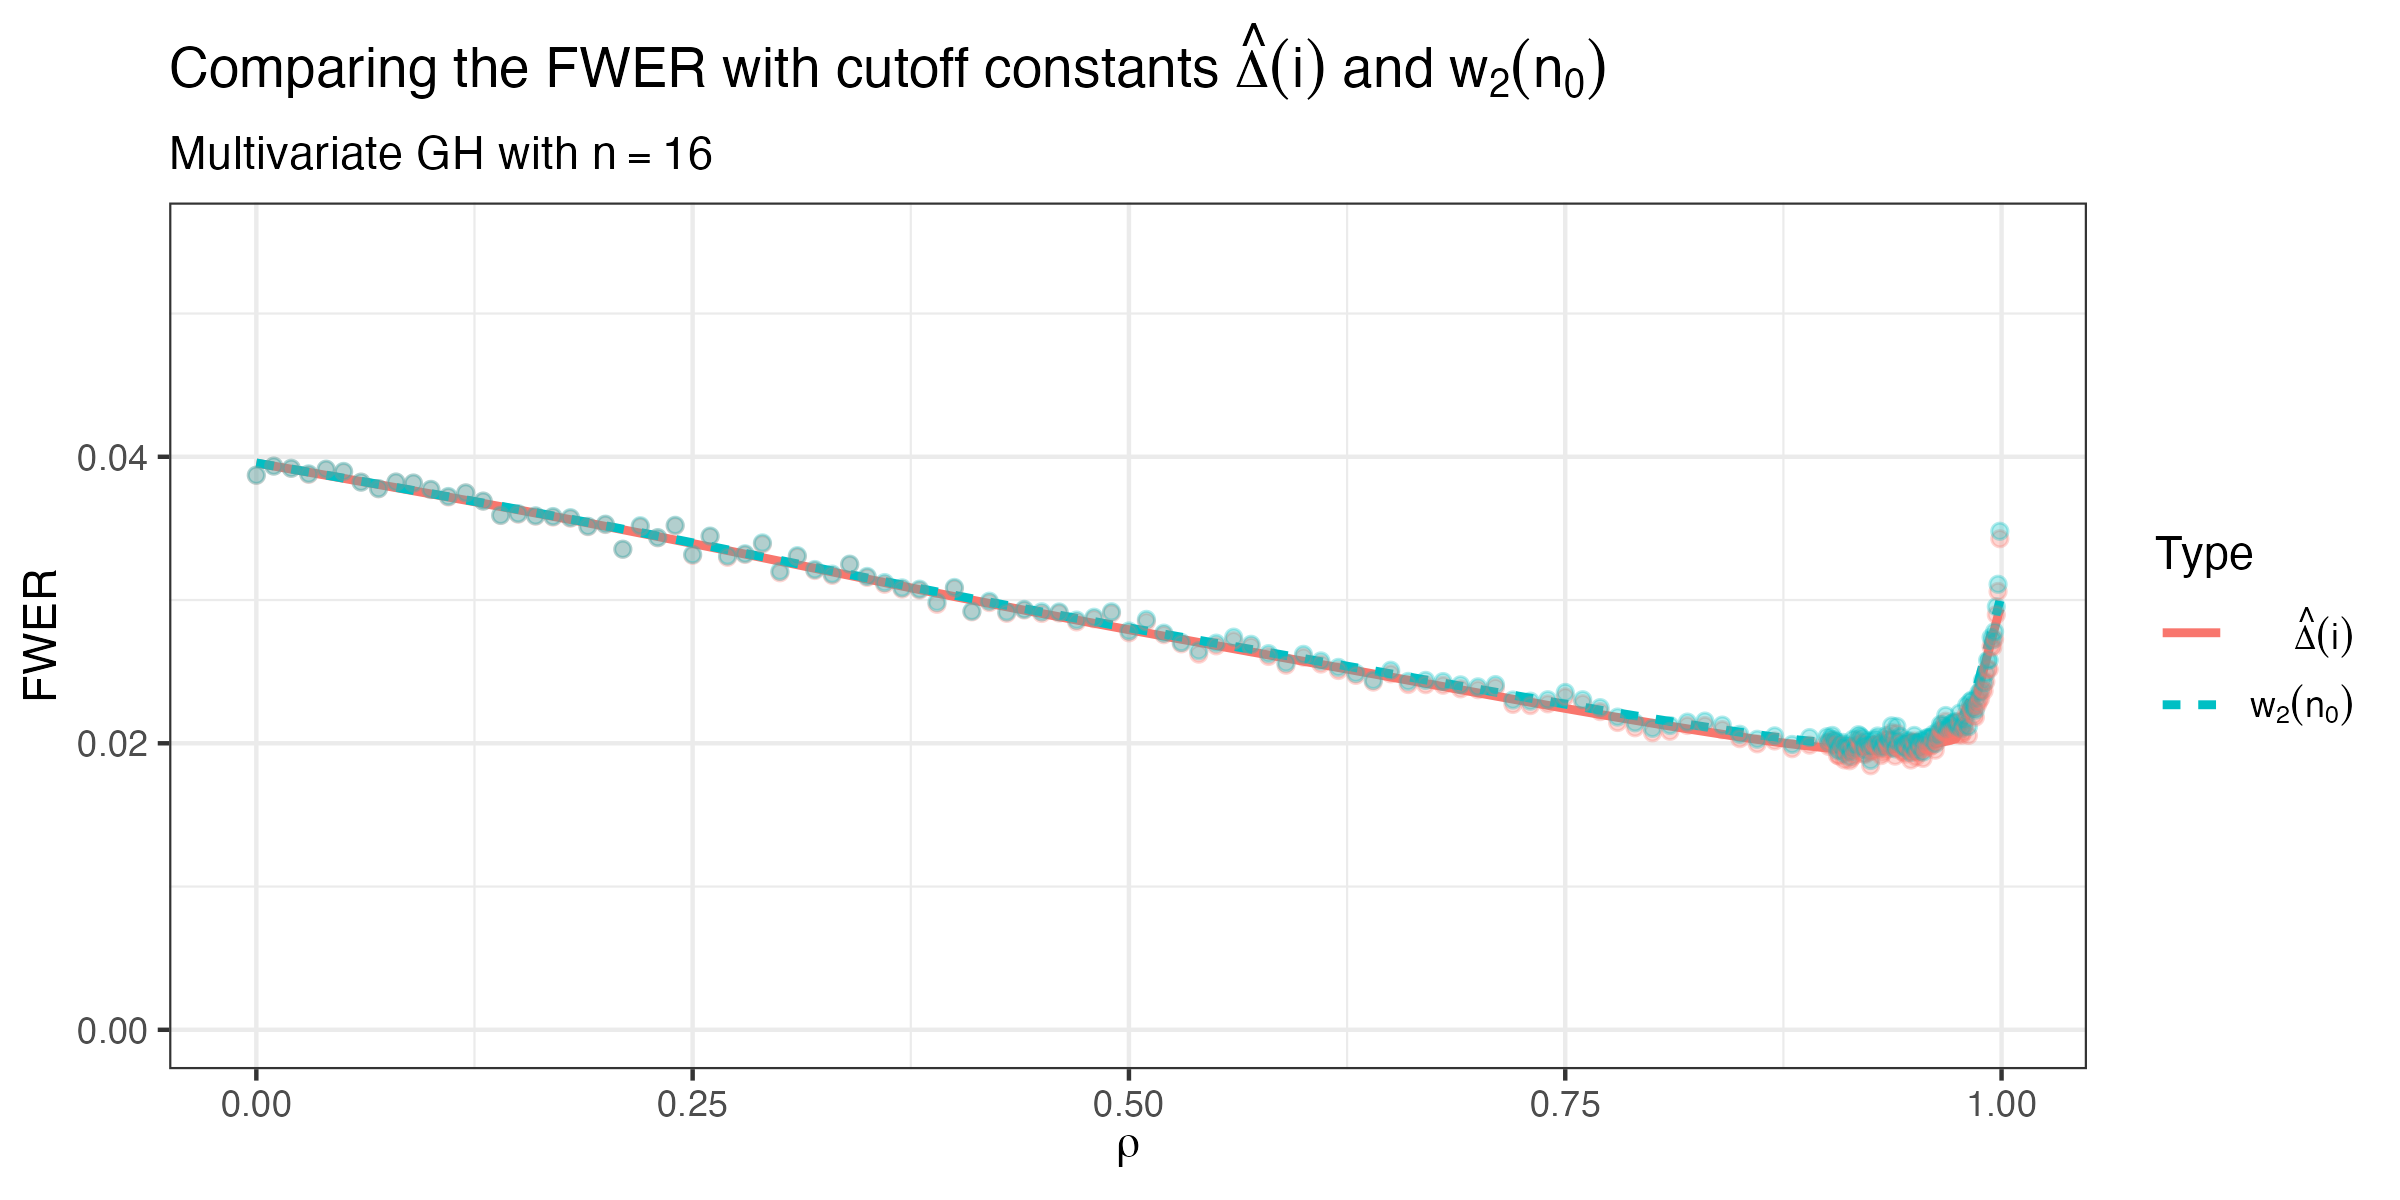
\includegraphics{figures/FWER_GH1_isi.png}}
\caption{Comparing the familywise error rate with cutoff constants $\hat{\Delta}(i)$ and $w_2(n_0)$}
\label{FWER_GH_comparison1}
\end{figure}


\bibliography{references}




\end{document}


